\section{SLTRs}

Wir wollen uns mit einer speziellen Darstellung planarer Graphen befassen bei der jedes Gebiet drei ausgewiesene Knoten, die Ecken, hat und alle anderen Knoten auf geraden Linien zwischen diesen Ecken liegen.

\begin{definition}[SLTR]\label{defsltr}
Eine Zeichnung eines planen Graphen $G$ wird Gradlinige Dreiecks Darstellung, im weiteren kurz \textit{SLTR} (kurz für die englische Bezeichnung Staight Line Triangle Representation), genannt falls gilt:
\begin{itemize}
\item[S1] Alle Kanten Segmente von Geraden
\item[S2] Alle Gebiete, inklusive dem äusseren, sind nicht degenerierte Dreiecke.
\end{itemize}
Wenn die Aufhängungen $s_1,s_2,s_3$ gegeben sind, dann sind diese auch die Ecken des äusseren Gebietes.
\end{definition}

\begin{figure}
	\centering
  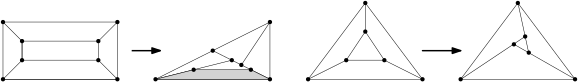
\includegraphics[scale=0.65]{sltr-example.png}
	\caption{Links der kleinste 3-zusammenhängende Graph, der kein SLTR hat und rechts ein Graph mit einer möglichen SLTR.}
	\label{cut_figure}
\end{figure}